Various template techniques sometimes cause a class template to end up with many different template type parameters. However, many of these parameters often have reasonable default values. A natural way to define such a class template may look as follows:

\begin{lstlisting}[style=styleCXX]
template<typename Policy1 = DefaultPolicy1,
		typename Policy2 = DefaultPolicy2,
		typename Policy3 = DefaultPolicy3,
		typename Policy4 = DefaultPolicy4>
class BreadSlicer {
	...
};
\end{lstlisting}

Presumably, such a template can often be used with the default template argument values using the syntax BreadSlicer<>. However, if a nondefault argument must be specified, all preceding arguments must be specified too (even though they may have the default value).

Clearly, it would be attractive to be able to use a construct akin to BreadSlicer<Policy3 = Custom> rather than BreadSlicer<DefaultPolicy1, DefaultPolicy2, Custom>, as is the case right now. In what follows we develop a technique to enable almost exactly that.

\begin{tcolorbox}[colback=webgreen!5!white,colframe=webgreen!75!black]
\hspace*{0.75cm}Note that a similar language extension for function call arguments was proposed (and rejected) earlier in the C++ standardization process (see Section 17.4 on page 358 for details).
\end{tcolorbox}

Our technique consists of placing the default type values in a base class and overriding some of them through derivation. Instead of directly specifying the type arguments, we provide them through helper classes. For example, we could write BreadSlicer<Policy3\_is<Custom>>. Because each template argument can describe any of the policies, the defaults cannot be different. In other words, at a high level, every template parameter is equivalent:

\begin{lstlisting}[style=styleCXX]
template<typename PolicySetter1 = DefaultPolicyArgs,
		typename PolicySetter2 = DefaultPolicyArgs,
		typename PolicySetter3 = DefaultPolicyArgs,
		typename PolicySetter4 = DefaultPolicyArgs>
class BreadSlicer {
	using Policies = PolicySelector<PolicySetter1, PolicySetter2,
									PolicySetter3, PolicySetter4>;
	// use Policies::P1, Policies::P2, ... to refer to the various policies
	...
};
\end{lstlisting}

The remaining challenge is to write the PolicySelector template. It has to merge the different template arguments into a single type that overrides default type alias members with whichever nondefaults were specified. This merging can be achieved using inheritance:

\begin{lstlisting}[style=styleCXX]
// PolicySelector<A,B,C,D> creates A,B,C,D as base classes
// Discriminator<> allows having even the same base class more than once
template<typename Base, int D>
class Discriminator : public Base {
};

template<typename Setter1, typename Setter2,
		typename Setter3, typename Setter4>
class PolicySelector : public Discriminator<Setter1,1>,
						public Discriminator<Setter2,2>,
						public Discriminator<Setter3,3>,
						public Discriminator<Setter4,4> {
};
\end{lstlisting}

Note the use of an intermediate Discriminator template. It is needed to allow the various Setter types to be identical. (You cannot have multiple direct base classes of the same type. Indirect base classes, on the other hand, can have types that are identical to those of other bases.)

As announced earlier, we’re collecting the defaults in a base class:

\begin{lstlisting}[style=styleCXX]
// name default policies as P1, P2, P3, P4
class DefaultPolicies {
	public:
	using P1 = DefaultPolicy1;
	using P2 = DefaultPolicy2;
	using P3 = DefaultPolicy3;
	using P4 = DefaultPolicy4;
};
\end{lstlisting}

However, we must be careful to avoid ambiguities if we end up inheriting multiple times from this base class. Therefore, we ensure that the base class is inherited virtually:

\begin{lstlisting}[style=styleCXX]
// class to define a use of the default policy values
// avoids ambiguities if we derive from DefaultPolicies more than once
class DefaultPolicyArgs : virtual public DefaultPolicies {
};
\end{lstlisting}

Finally, we also need some templates to override the default policy values:

\begin{lstlisting}[style=styleCXX]
template<typename Policy>
class Policy1_is : virtual public DefaultPolicies {
	public:
	using P1 = Policy; // overriding type alias
};

template<typename Policy>
class Policy2_is : virtual public DefaultPolicies {
	public:
	using P2 = Policy; // overriding type alias
};

template<typename Policy>
class Policy3_is : virtual public DefaultPolicies {
	public:
	using P3 = Policy; // overriding type alias
};

template<typename Policy>
class Policy4_is : virtual public DefaultPolicies {
	public:
	using P4 = Policy; // overriding type alias
};
\end{lstlisting}

With all this in place, our desired objective is achieved. Now let’s look at what we have by example. Let’s instantiate a BreadSlicer<> as follows:

\begin{lstlisting}[style=styleCXX]
BreadSlicer<Policy3_is<CustomPolicy>> bc;
\end{lstlisting}

For this BreadSlicer<> the type Policies is defined as

\begin{lstlisting}[style=styleCXX]
PolicySelector<Policy3_is<CustomPolicy>,
				DefaultPolicyArgs,
				DefaultPolicyArgs,
				DefaultPolicyArgs>
\end{lstlisting}

With the help of the Discriminator<> class templates, this results in a hierarchy in which all template arguments are base classes (see Figure 21.4). The important point is that these base classes

\begin{center}
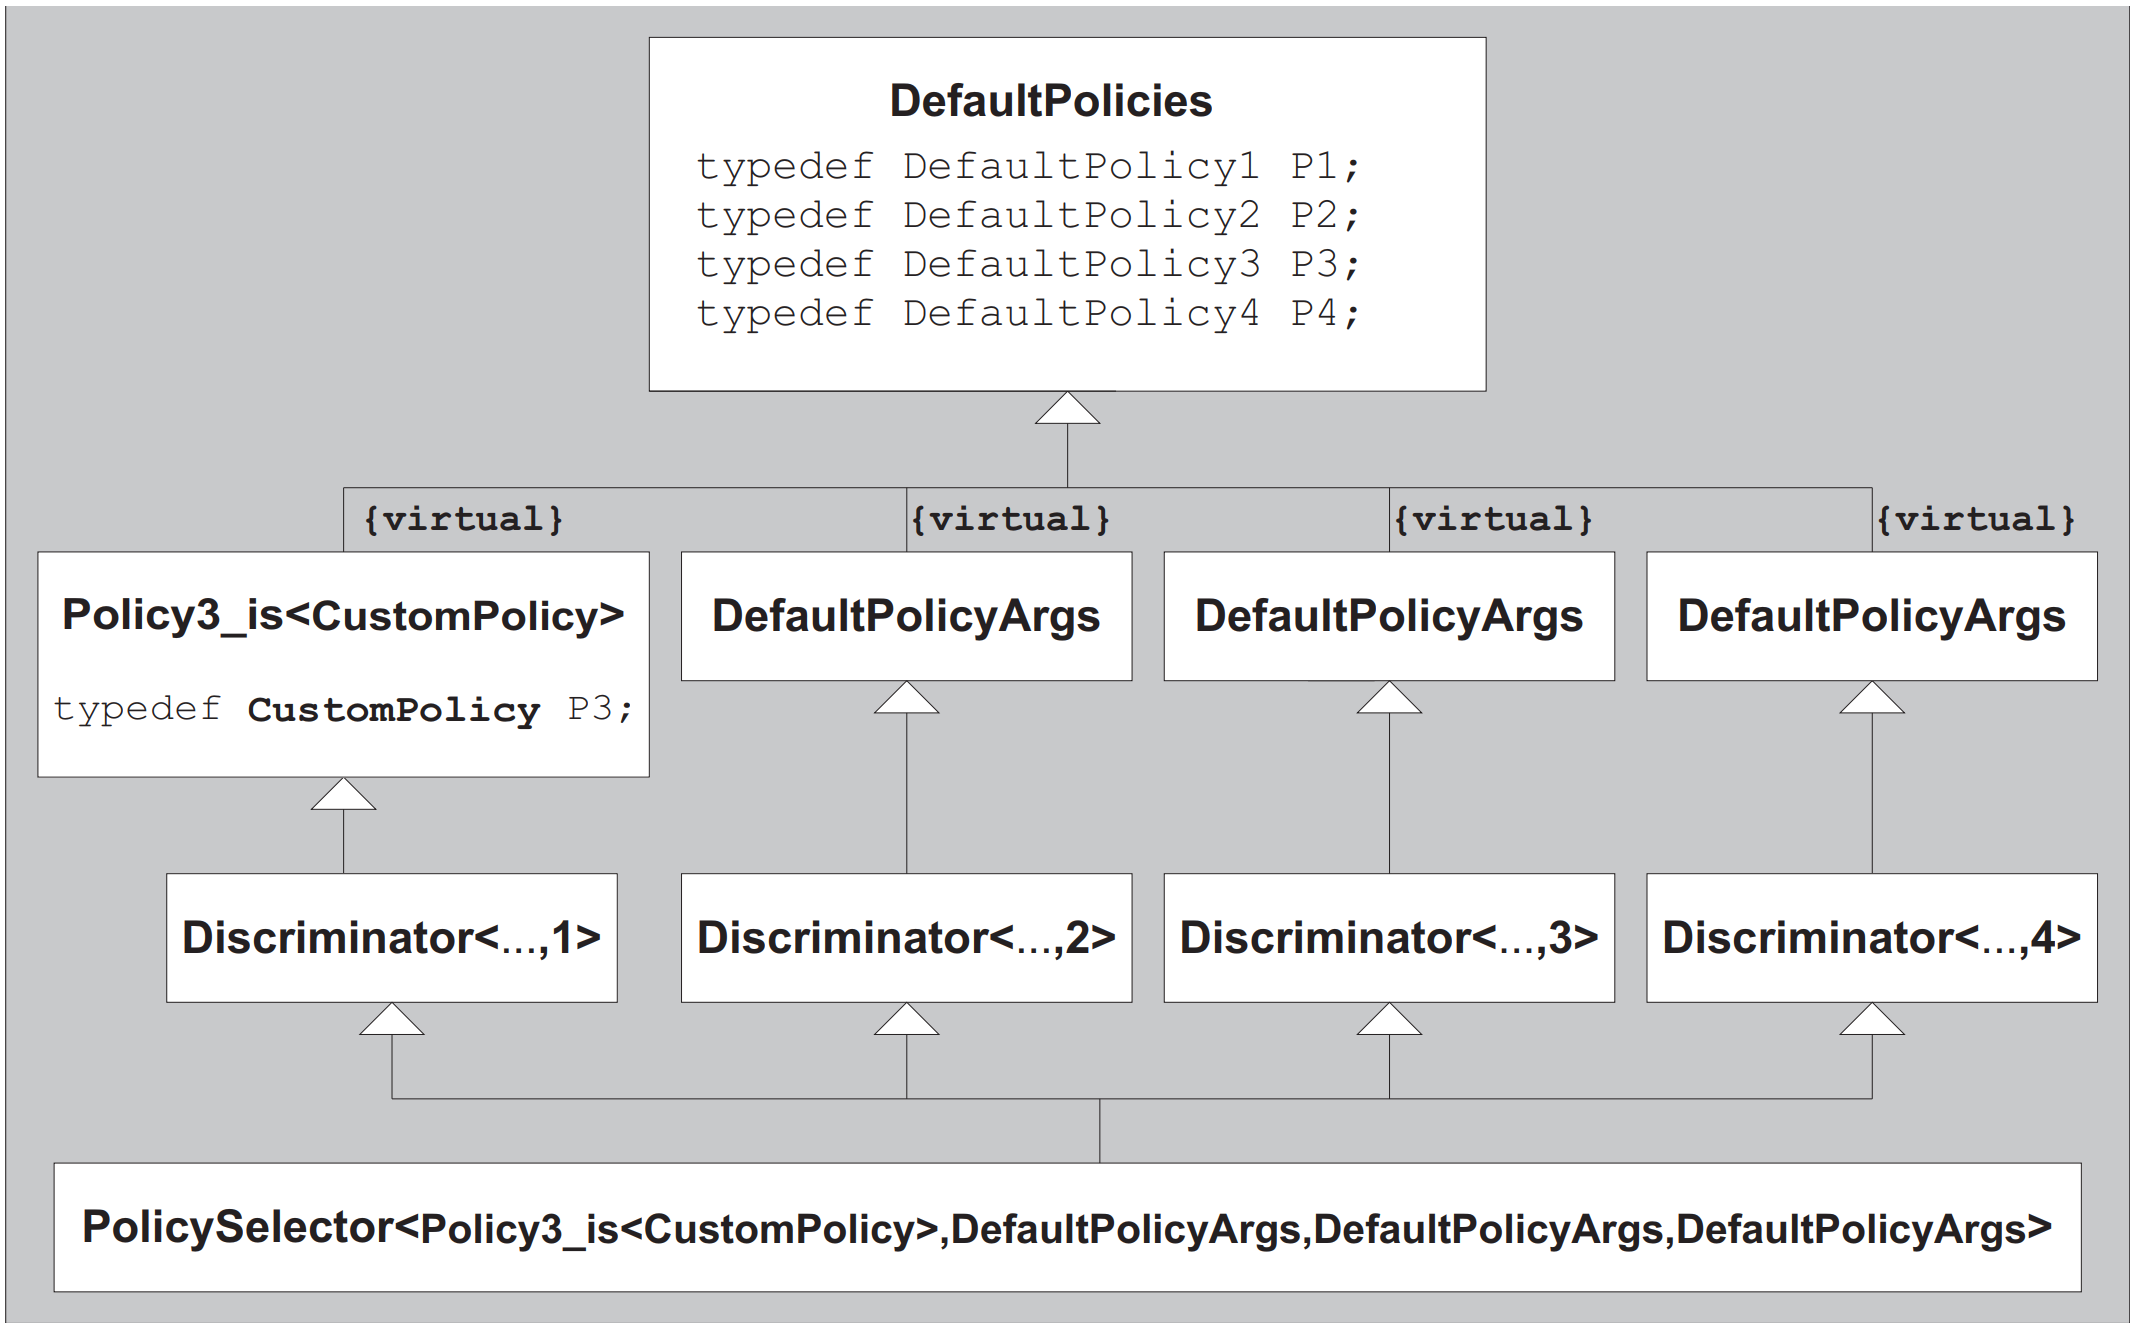
\includegraphics[width=0.8\textwidth]{content/3/chapter21/images/4.png} \\
Figure 21.4. Resulting type hierarchy of BreadSlicer<>::Policies
\end{center}

all have the same virtual base class DefaultPolicies, which defines the default types for P1, P2, P3, and P4. However, P3 is redefined in one of the derived classes—namely, in Policy3\_is<>. According to the domination rule, this definition hides the definition of the base class. Thus, this is not an ambiguity.

\begin{tcolorbox}[colback=webgreen!5!white,colframe=webgreen!75!black]
\hspace*{0.75cm}You can find the domination rule in Section 10.2/6 in the first C++ standard (see [C++98]) and a discussion about it in Section 10.1.1 of [EllisStroustrupARM].
\end{tcolorbox}

Inside the template BreadSlicer you can refer to the four policies by using qualified names such as Policies::P3. For example:

\begin{lstlisting}[style=styleCXX]
template<...>
class BreadSlicer {
	...
	public:
	void print () {
		Policies::P3::doPrint();
	}
	...
};
\end{lstlisting}

In inherit/namedtmpl.cpp you can find the entire example.

We developed the technique for four template type parameters, but it obviously scales to any reasonable number of such parameters. Note that we never actually instantiate objects of the helper class that contain virtual bases. Hence, the fact that they are virtual bases is not a performance or memory consumption issue.






